\section{Foundations}

\begin{frame}[c]
\Huge{\centerline{Foundations}}
\end{frame}

%----------------------------------------------------------------------------------------

\begin{frame}\frametitle{Introduction \& Purpose}
	\begin{itemize}
		\item \textbf{Goal:} Ability to interpret complex "black box" models, deemed uninterpretable for decades.
		\bigskip 
		\item \textbf{Solution:} Some approaches that increase a complex model's transparency, accountability, and fairness are the following:
		\bigskip
		\begin{itemize}
			\item Decision tree surrogate models [\cite{dt_surrogate1}; \cite{dt_surrogate2}]
			\item Partial dependence plots [\cite{esl}]
			\item Individual conditional expectation (ICE) plots [\cite{ice_plots}]
			\item Random forest feature importance [\cite{esl}]
			\item Leave-one-covariate-out (LOCO) local feature importance [\cite{conformal_reg}]
			\item Local Interpretable Model-agnostic Explanations (LIME) [\cite{lime}]
			\item Shapley Explanations [\cite{shapley}; \cite{tree_shap}]
			\end{itemize}
	\end{itemize}
\end{frame}
%----------------------------------------------------------------------------------------

\begin{frame}\frametitle{Introduction \& Purpose}
	\begin{itemize}
		\item The following slides will detail the mathematics behind each of these approaches and techniques. 
	\end{itemize}
\end{frame}

%----------------------------------------------------------------------------------------

\begin{frame}\frametitle{Notation \& Preliminaries}
	\begin{itemize}
		\item \textbf{Spaces}.  
			\begin{itemize}
				\item The input features come from a set  $\mathcal{X}$ contained in a \textit{P}-dimensional input space (i.e. $\mathcal{X} \subset \mathbb{R}^P)$.  
				\item The output responses come from a set $\mathcal{Y}$ contained in a $C$-dimensional output space (i.e. $\mathcal{Y} \subset \mathbb{R}^C$).
			\end{itemize}	
			\bigskip	
		\item \textbf{Dataset}. A dataset $\mathbf{D}$ consists of $N$ tuples of observations:\\ $[(\mathbf{x}^{(0)},\mathbf{y}^{(0)}), (\mathbf{x}^{(1)},\mathbf{y}^{(1)}), \dots, (\mathbf{x}^{(N-1)},\mathbf{y}^{(N-1)})], \mathbf{x}^{(i)} \in \mathcal{X}, \mathbf{y}^{(i)} \in \mathcal{Y}$.\\
			\begin{itemize}
			\item The input data $\mathbf{X}$ is composed of the set of row vectors $\mathbf{x}^{(i)}$. 
				\begin{itemize}
					\item let $\mathcal{P}$ be the set of features  $\{X_0, X_1, \dots, X_{P-1}\}$, where $X_j = \left[x_{j}^{(0)}, x_{j}^{(1)}, \dots, x_{j}^{(N-1)} \right]^T$.
					\item then each $i$-th observation denoted as $\mathbf{x}^{(i)} = \left[x_0^{(i)}, x_1^{(i)}, \dots, x_{P-1}^{(i)} \right]$ is an instance of $\mathcal{P}$.
				\end{itemize}
		\end{itemize}
	\end{itemize}
\end{frame}
%----------------------------------------------------------------------------------------

\begin{frame}\frametitle{Preliminaries (Cont.)}
	\begin{itemize}
		\item \textbf{Learning Problem}. We want to discover some \textit{unknown target function} $f: \mathcal{X} \rightarrow \mathcal{Y}$ from our data $\mathbf{D}$, which we assume is identically and independently distributed (i.i.d).  To do so, we explore a \textit{hypothesis set} $\mathcal{H}$ and use a given learning algorithm $\mathcal{A}$ to find a function $g$ that we hope sufficiently approximates our target function: $\mathbf{D} \xrightarrow[]{\mathcal{A}} g \approx f$.  For a given training example $(\mathbf{x}, \mathbf{y})$ in $\mathbf{D}$, we hope that $g(\mathbf{x}) = \hat{\mathbf{y}} \approx \mathbf{y}$ and $g$ generalizes well for unseen observations.
	\end{itemize}
\end{frame}

%----------------------------------------------------------------------------------------

\begin{frame}\frametitle{Preliminaries (Cont.)}
	\begin{figure}[htb]
	\begin{center}
		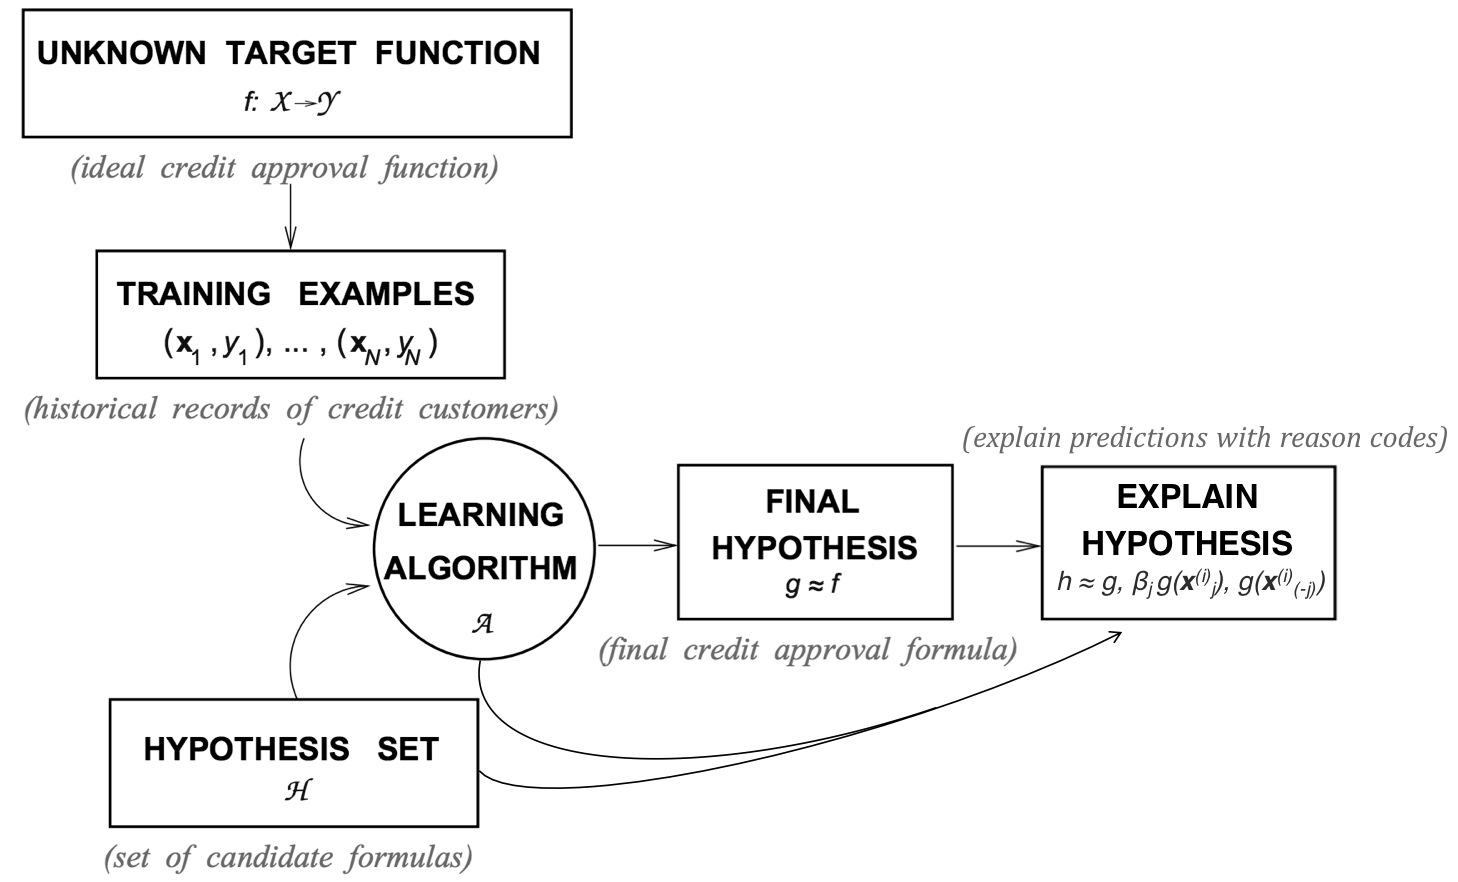
\includegraphics[width=0.77\textwidth]{images/learning_problem.png}
		\caption{The learning problem. Adapted from \textbf{Learning From Data}.}
		\label{fig:learning_problem}
	\end{center}
	\end{figure}
\end{frame}

%----------------------------------------------------------------------------------------

\begin{frame}\frametitle{Preliminaries (Cont.)}
	\begin{itemize}
		\item \textbf{Explanation}. To justify the predictions of $g(\mathbf{x})$, we may resort to a number of techniques. Some techniques will be global in scope and simply seek to generate an interpretable approximation, $h$, for $g$ itself, such that $h(\mathbf{x}) \approx g(\mathbf{x}) = \hat{\mathbf{y}}(\mathbf{x})$. Other techniques will be more local in scope and attempt to rank local contributions for each feature $X_j \in \mathcal{P}$ for some observation $\mathbf{x}^{(i)}$; this can create reason codes for $g(\mathbf{x}^{(i)})$. Local contributions are often estimated by evaluating the product of a learned parameter $\beta_j$ in $g$ with a corresponding observed feature value $x_j^{(i)}$ (i.e. $\beta_jx_j^{(i)}$), or by seeking to remove the contribution of some $X_j$ in a prediction, $g(\mathbf{x}_{(-j)}^{(i)})$.
	\end{itemize}
\end{frame}




